% Name: d orbitals
% Description: Three of the five d orbitals, dxy, dx²−y², and dz², each labeled, with the phases of their lobes shaded in two colors.
% Tags: d orbitals, atomic orbitals, transition metals, quantum chemistry

\usepackage{tikzorbital}

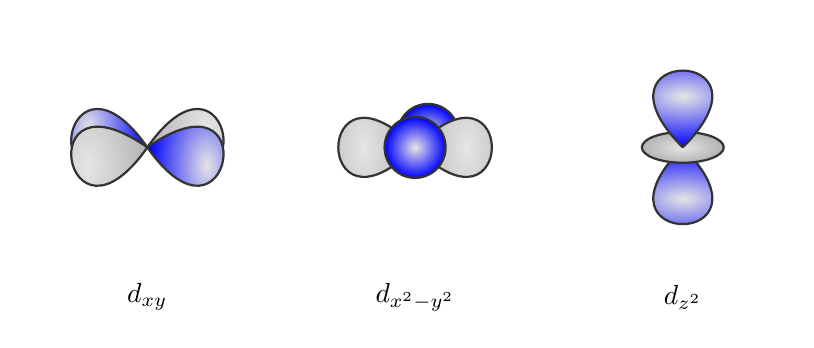
\begin{tikzpicture}
  \foreach \o/\l [count=\i from 0] in {dxy/{d_{xy}}, dx2y2/{d_{x^2-y^2}}, dz2/{d_{z^2}}} {
    \begin{scope}[shift={(3.4*\i,0)}]
      \orbital[scale=1.3]{\o}
      \node at (0,-1.9) {$\l$};
    \end{scope}
  }
\end{tikzpicture}
